\chapter{实验三:数据并行}

\section{实验内容与要点介绍}

\subsection{实验内容与要求}

\subsubsection{实验内容}
\begin{itemize}
    \item 学习掌握分布式策略中的数据并行训练策略
    \item 掌握数据并行的原理
    \item 掌握常用的数据划分策略
    \item 构建随机采样和随机划分方式将数据集分发到不同的设备,并进行模型训练
\end{itemize}


\subsubsection{实验要求}
\begin{itemize}
    \item 模拟多节点的DML系统,将一个完整数据集以不同的划分方式划分,并分配给系统中的节点。
    \item 实现包括随机采样和随机划分的划分方式,并实现数据并行地训练模型
    \item 分析数据并行相对于单机训练的性能指标提升,分析不同数据划分方法对模型性能的影响
\end{itemize}


\subsection{数据集、加载器和采样器}

在Pytorch中,分布式训练加载数据过程中涉及到这样三个重要的类,即\graylstinline{Dataset}、\graylstinline{Sampler}、\graylstinline{DataLoader}:
\begin{itemize}
    \item \graylstinline{Dataset}类:它直接接触源数据,将数据总数目交给\graylstinline{Sampler},将提取数据的接口交给\graylstinline{Dataloader}。
    \item \graylstinline{Sampler}类:定义\graylstinline{DataLoader}遍历数据索引的方式。
    \item \graylstinline{DataLoader}类:在得到\graylstinline{Sampler}提供的数据索引后,去\graylstinline{Dataset}中提取数据,并将得到的数据用于训练。
\end{itemize}

他们之间的关系可以用图\ref{fig:task3-sampler-dataset-dataloader}来表示。
\begin{figure}[htbp]
	\centering
	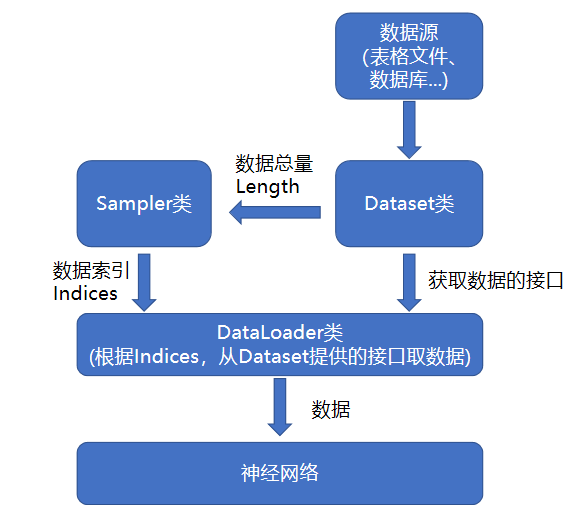
\includegraphics[width=0.7\textwidth]{figures/task3-sampler-dataset-dataloader.png}
	\caption{caption:task3-sampler-dataset-dataloader}
	\label{fig:task3-sampler-dataset-dataloader}
\end{figure}

在我们的实验中,我们主要需要实现\graylstinline{Sampler}类,除了构造函数外,还需要实现该类中的\graylstinline{__iter__()}方法和\graylstinline{__len__()}方法。
在\graylstinline{__iter__()}方法中,需要返回包含样本序列号的一个迭代器,譬如,一段最简单的迭代器可以这样实现:
\begin{lstlisting}
def __iter__(self):
    indices=list(range(len(self.dataset)))
    return iter(indices)
\end{lstlisting}

\graylstinline{__len__()}方法则应当返回上述迭代器中的数据个数。除此之外,我们也可以尝试在\graylstinline{Sampler}中实现其他功能,譬如\graylstinline{set_epoch()}方法,并在每一轮训练前调用该方法,以避免每一轮训练都得到同样的indices序列。


在本实验中,同学们可以利用实验2中学到的知识,尝试使用\graylstinline{multiprocessing}或自己编写docker-compose.yaml来模拟多节点~

